\section{Approach \& Experiments}
\begin{frame}{Improving OpenMax}
	\begin{itemize}
		\item Handling negative logits
		      \begin{itemize}
			      \item Value Shift
			      \item Adjust Probabilities
		      \end{itemize}
		\item Introducing weight factors
		      \begin{itemize}
			      \item $ \phi_N = \frac{1}{N-1}$
			      \item $ \phi_{\omega} = \frac{1}{\sum_i (1 - \omega_i)}$
		      \end{itemize}
		\item Removing alpha parameter
	\end{itemize}
\end{frame}

\begin{frame}{Research Questions 1}
	\texttt{RQ1}: Can OpenMax performance be enhanced by accounting for negative activation values?
\end{frame}

\begin{frame}{Open-Set Classification Rate}
	Correct Classification Rate (CCR)
	\begin{itemize}
		\item Known samples
		\item Threshold $\theta$
		      \begin{equation}
			      \operatorname{CCR} (\theta) = \frac{| \{ k_{c} | \operatorname{argmax}_{1 \leq n \leq N} y_{c,n} = \tau_{c} \wedge y_{c,n} \geq \theta \}|}{ |K|}
		      \end{equation}
	\end{itemize}
	False Positive Rate (FPR)
	\begin{itemize}
		\item Unknown samples
		\item Threshold $\theta$
		      \begin{equation}
			      \operatorname{FPR}(\theta) = \frac{| \{ u_{c} | \operatorname{argmax}_{1 \leq n \leq N} y_{c,n} \geq \theta \}|}{ |U|}
		      \end{equation}
	\end{itemize}
\end{frame}

\begin{frame}{Defining Scoring System}
	\begin{itemize}
		\item $\Sigma$-Score - Thresholding
		\item $\gamma$-Score $ \gamma = \frac{(\gamma^+ + \gamma^-)}{2}$
		      \begin{equation}
			      \gamma^+ = \frac{1}{|K|} \sum_{c=1}^{|K|} y_{\tau_c}
		      \end{equation}
		      \begin{equation}
			      \gamma^- = \frac{1}{|U|} \sum_{c=1}^{|U|} \left ( 1 - \operatorname{argmax}_{1 \leq n \leq N} y_{c,n} \right)
		      \end{equation}
	\end{itemize}
\end{frame}

\begin{frame}{Baseline ($\gamma$)}
	\centering
	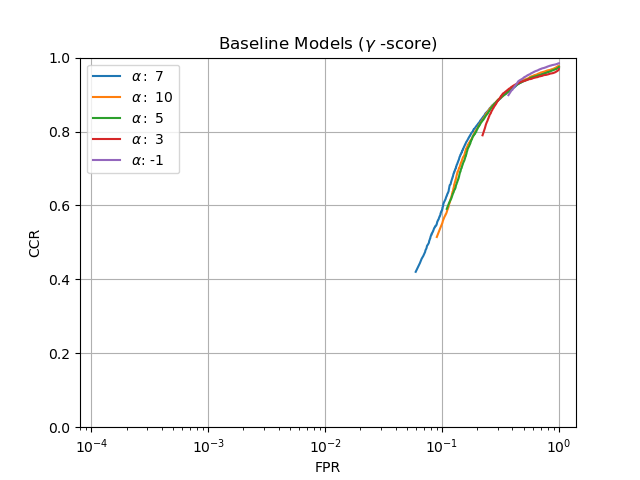
\includegraphics[width=0.65\textwidth]{figures/base_gamma.png}
	\footnotesize{	\begin{tabularx}{\textwidth}{ |X|X|X|X|X|X| }
			\hline
			Rank & $\alpha$ & $\eta$ & $\kappa$ & $\gamma$ & $\Sigma$ \\
			\hline
			1    & 7        & 1000   & 1.0      & 0.805    & 4.272    \\
			2    & 10       & 1000   & 1.0      & 0.803    & 3.685    \\
			3    & 5        & 1000   & 1.0      & 0.800    & 3.669    \\
			4    & 3        & 1000   & 1.0      & 0.718    & 2.855    \\
			5    & -1       & 1000   & 1.0      & 0.600    & 2.899    \\
			\hline
		\end{tabularx}}
\end{frame}

\begin{frame}{Baseline ($\Sigma$)}
	\centering
	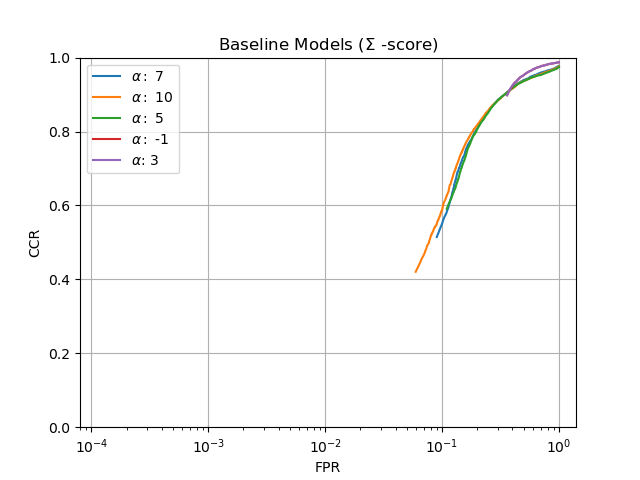
\includegraphics[width=0.65\textwidth]{figures/base_sigma.png}
	\footnotesize{	\begin{tabularx}{\textwidth}{ |X|X|X|X|X|X| }
			\hline
			Rank & $\alpha$ & $\eta$ & $\kappa$ & $\gamma$ & $\Sigma$ \\
			\hline
			1    & 7        & 1000   & 1.0      & 0.805    & 4.272    \\
			2    & 10       & 1000   & 1.0      & 0.803    & 3.685    \\
			3    & 5        & 1000   & 1.0      & 0.800    & 3.669    \\
			4    & -1       & 10     & 2.3      & 0.514    & 2.917    \\
			5    & 3        & 100    & 3.0      & 0.514    & 2.916    \\
			\hline
		\end{tabularx}
	}
\end{frame}

\begin{frame}{Results RQ1 ($\gamma$)}
	\centering
	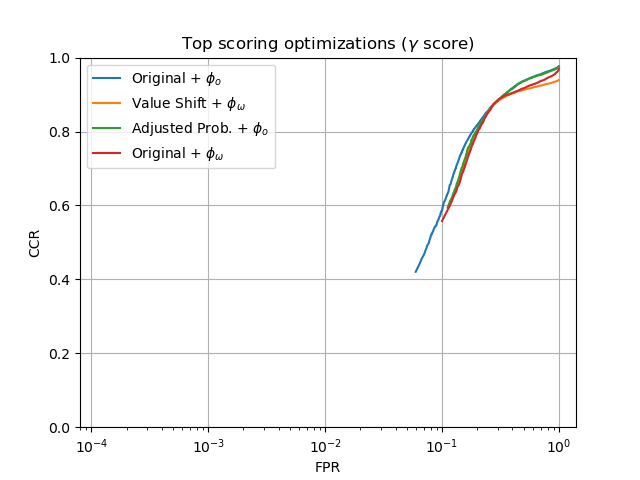
\includegraphics[width=0.65\textwidth]{figures/Top-gamma.png}
	\footnotesize{\begin{tabularx}{\textwidth}{ |X|X|X|X|X|l|X|X| }
			\hline
			Rank & $\alpha$ & $\eta$ & $\kappa$ & $\phi$        & Negative fix   & $\gamma$ & $\Sigma$ \\
			\hline
			1    & 7        & 1000   & 1.0      & $\phi_o$      & Original       & 0.805    & 4.272    \\
			2    & 5        & 1000   & 1.0      & $\phi_\omega$ & Value Shift    & 0.801    & 3.578    \\
			3    & 5        & 1000   & 1.0      & $\phi_o$      & Adjusted Prob. & 0.801    & 3.671    \\
			4    & 3        & 1000   & 1.0      & $\phi_\omega$ & Original       & 0.792    & 4.176    \\
			\hline
		\end{tabularx}
	}
\end{frame}

\begin{frame}{Results RQ1 ($\Sigma$)}
	\centering
	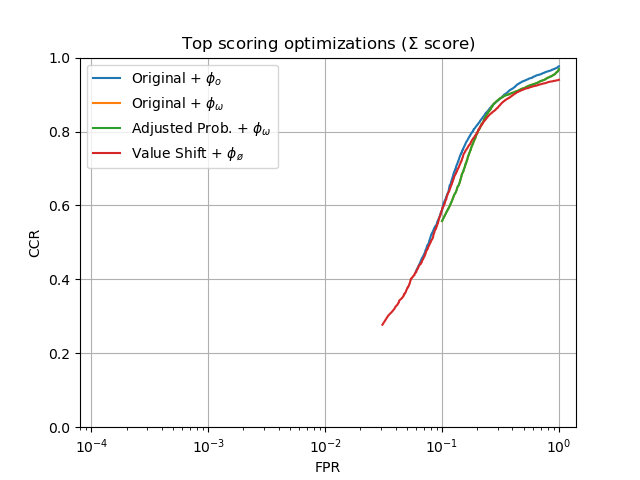
\includegraphics[width=0.65\textwidth]{figures/Top-sigma.png}
	\footnotesize{   \begin{tabularx}{\textwidth}{ |X|X|X|X|X|l|X|X| }
			\hline
			Rank & $\alpha$ & $\eta$ & $\kappa$ & $\phi$        & Negative fix   & $\gamma$ & $\Sigma$ \\
			\hline
			1    & 7        & 1000   & 1.0      & $\phi_o$      & Original       & 0.805    & 4.272    \\
			2    & 3        & 1000   & 1.0      & $\phi_\omega$ & Original       & 0.792    & 4.176    \\
			3    & 3        & 1000   & 1.0      & $\phi_\omega$ & Adjusted Prob. & 0.792    & 4.176    \\
			4    & 5        & 1000   & 1.0      & $\phi_o$      & Value Shift    & 0.749    & 4.169    \\
			\hline
		\end{tabularx}}
\end{frame}

\begin{frame}{Where to apply the clustering?}
	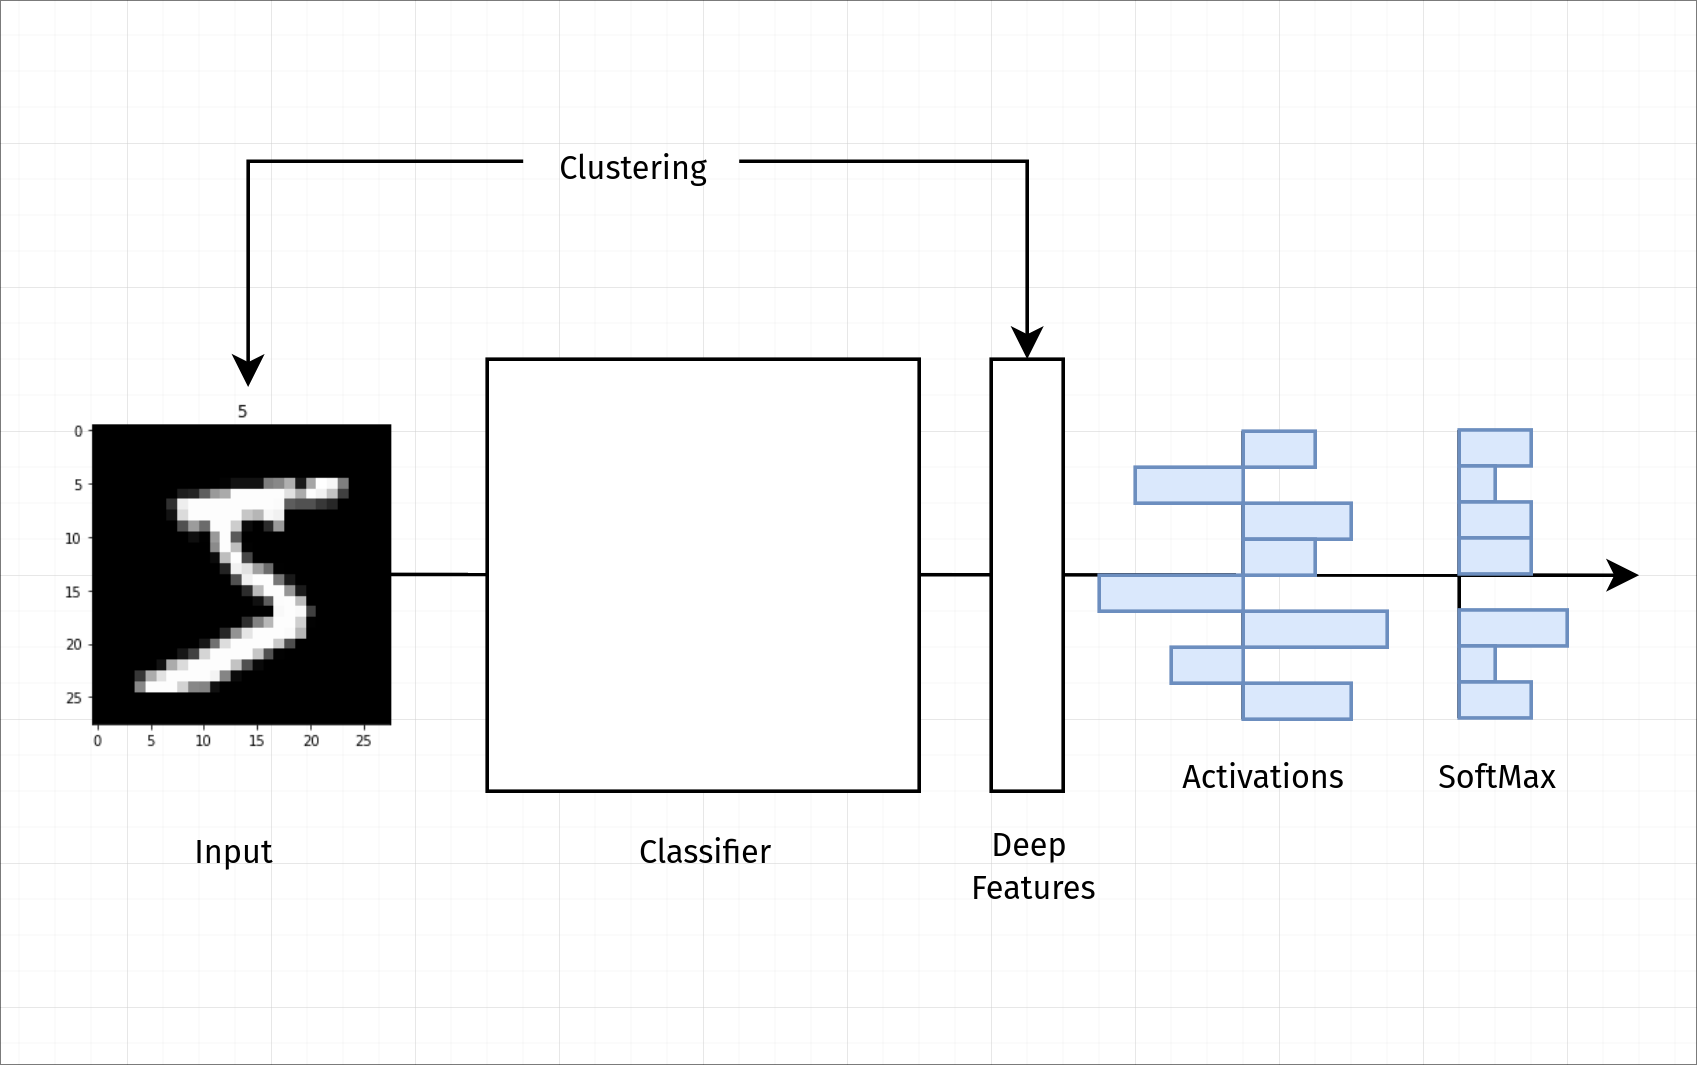
\includegraphics[width=\textwidth]{figures/openmax_clustering.png}
\end{frame}

\begin{frame}{Introducing Clustering to OpenMax}
	Input Clustering:
	\begin{itemize}
		\item Input data
		\item Per class
		\item Each cluster a class
	\end{itemize}
	Features Clustering:
	\begin{itemize}
		\item Training Features
		\item Validation Features
		\item Per class
	\end{itemize}
	Combination of both types
\end{frame}

\begin{frame}{Visualizing Clustering}
	\centering
	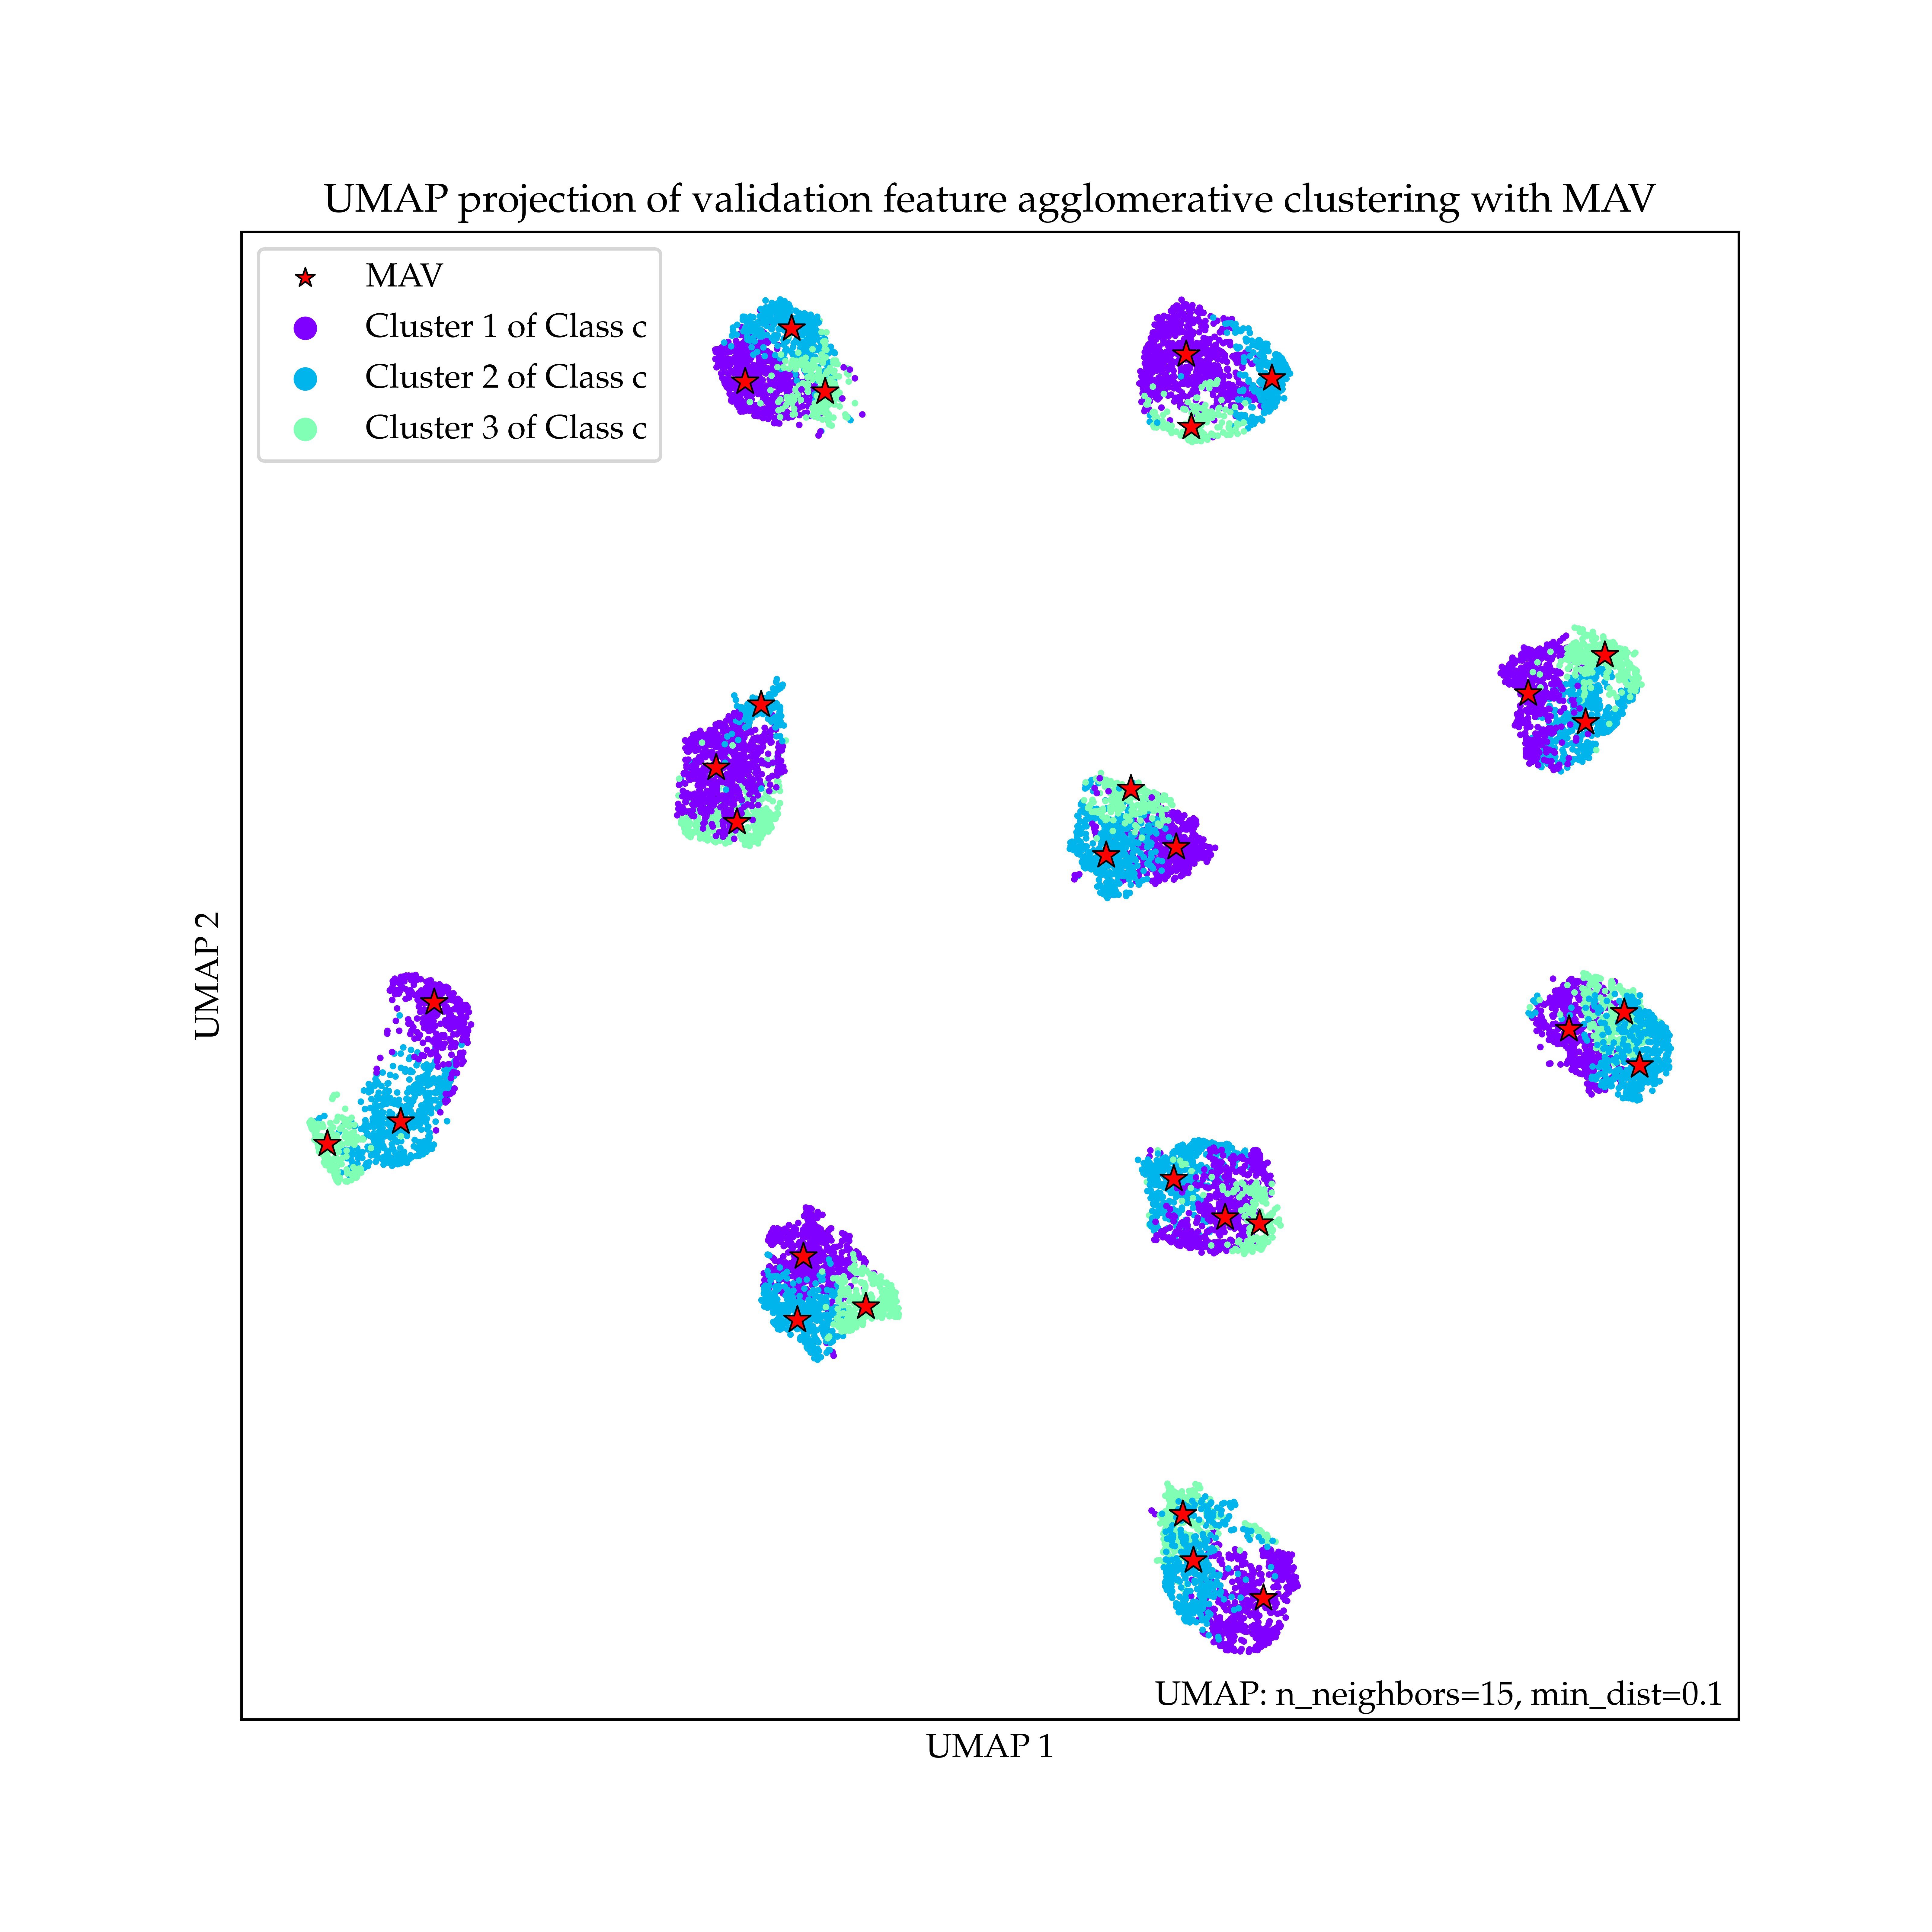
\includegraphics[width=0.75\textwidth]{figures/umap_projection_emnist_cluster.png}
\end{frame}
